% Description: Cours de programmation sous SIG

% Modules generaux
\documentclass[11pt]{article}
\usepackage[utf8]{inputenc}
\usepackage[T1]{fontenc}
\usepackage[francais]{babel} % prise en charge du francais
\usepackage[table]{xcolor} % tableaux
\usepackage{graphicx} % images
\usepackage{float}
\usepackage[font=small]{caption}

% Marges
\usepackage[left=2cm,right=2cm,top=2cm,bottom=2cm]{geometry}

% Personnalisation des titres
\usepackage{titlesec}
\titlespacing{\section}{0em}{4em}{1em}
\titlespacing{\subsection}{0em}{2em}{0em}
\titlespacing{\subsubsection}{0em}{0.5em}{0em}

% Mise en page
\setlength{\parskip}{1.2em}
\renewcommand{\floatpagefraction}{1}

% Couleurs personnalisées
\usepackage{color}
\definecolor{lightgray}{gray}{0.98}
\definecolor{gray}{rgb}{0.6, 0.6, 0.65}
\definecolor{green}{rgb}{0.133, 0.545, 0.133}
\definecolor{blue}{rgb}{0, 0, 1}
\definecolor{red}{rgb}{0.6, 0.1, 0.1}

% Liens hypertextes
\usepackage{hyperref}
\hypersetup{
	colorlinks=true,
	breaklinks=true,
	urlcolor=blue,
	linkcolor=blue,
	pdfborder=000,
	pdftex=true
}

% Mise en forme des codes python
\usepackage{listingsutf8}
\lstset{
	language=python,
	inputencoding=utf8/latin1,
	extendedchars=true,
	keywordstyle=\bfseries\ttfamily\color{blue},
	identifierstyle=\ttfamily,
	commentstyle=\color{gray},
	stringstyle=\ttfamily\color{green},
	showstringspaces=false,
	basicstyle=\footnotesize\ttfamily,
	tabsize=2,
	breaklines=true,
	extendedchars=true,
	xleftmargin=1cm, 
	xrightmargin=1cm,
	backgroundcolor=\color{lightgray},
	literate=%
		{é}{{\'{e}}}1
		{è}{{\`{e}}}1
		{ê}{{\^{e}}}1
		{ë}{{\¨{e}}}1
		{û}{{\^{u}}}1
		{ù}{{\`{u}}}1
		{â}{{\^{a}}}1
		{à}{{\`{a}}}1
		{î}{{\^{i}}}1
		{ô}{{\^{o}}}1
		{ç}{{\c{c}}}1
}

% Commandes personnalisées
\newcommand{\bslash}{\texttt{\symbol{92}}}
\newcommand{\action}{$\Rightarrow$ }
\newcommand{\reponse}{\begin{tabbing}
\hspace{2cm}\=\kill
Réponse \> ............................................................................................ \\ 
 \> ............................................................................................
\end{tabbing}
}
\newenvironment{note}{%
	\begin{tabular}[t t]{c c}
		
\includegraphics{img/tips.png} &
		\begin{minipage}[c]{0.9\linewidth}
}{%
		\end{minipage}
	\end{tabular}
}

\newcommand{\code}[1]{\lstinline{#1}}

\newenvironment{python}{%
	\begin{lstlisting}
}{%
	\end{lstlisting}
}


%%%%%%%%%%%%%%%%%%%%%%%%%%%%%%%%%
% Infos générales sur le document
%%%%%%%%%%%%%%%%%%%%%%%%%%%%%%%%%
\title{Introduction à la programmation sous SIG}
\author{Clément Delgrange}
\date{\today}

% Entetes et pieds de page
\usepackage{fancyhdr}
\pagestyle{fancy}
\fancyhf{}
\renewcommand{\headrulewidth}{0pt}
\fancyfoot[L]{ENSG}
\fancyfoot[C]{-\thepage-}
\fancyfoot[R]{Programmation sous SIG}
\renewcommand{\footrulewidth}{0.5pt}


%%%%%%%%%%%%
%%% Document
%%%%%%%%%%%%
\begin{document}
	
	
% Création de la page de titre
\begin{titlepage}
	\begin{sffamily}
		\begin{flushleft}
			
\includegraphics[scale=0.15]{img/cours/logo_ensg.png}\\[1.5cm]
		\end{flushleft}
		\begin{flushright}
			% pour mettre une image en haut à droite
		\end{flushright}
		
		\vspace{1cm}
		
		\begin{center}
			\hrule
				\vspace{0.5cm}
				{\LARGE \bfseries Introduction à la programmation sous SIG}
				\vspace{0.7cm}
			\hrule
			
			\vspace{3cm}
			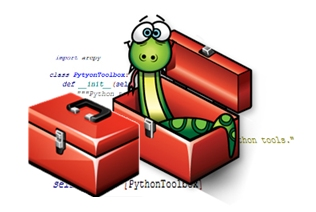
\includegraphics[width=0.5\textwidth]{img/cours/img1.jpg}
			\vspace{4cm}
		
			\large \textit{ENSG}\\
			\small \textit{Septembre 2017}
		\end{center}
	\end{sffamily}
\end{titlepage}


% Insertion de la table des matières
\addtocontents{toc}{
	\protect\setlength{\parskip}{0pt}
}
\tableofcontents
\newpage


%%%%%%%%%%%%%%%%%%%%%%%%%
% Début du corps du texte

\section{Introduction}
Les SIG s'adressent à des communautés d'utilisateurs très diverses. Bien que présentant des caractéristiques communes, ces outils doivent dans le détail apporter des solutions personnalisées à chacune d'entre elles. Cela est rendu possible par le développement logiciel. Une formation aux SIG doit donc nécessairement comporter un volet consacré à la programmation de tels systèmes.

L'évolution récente du monde de l'information géographique vers la mise en ligne de données et de services (sur le web ou bien au sein de réseaux d'entreprises) a renforcé l'importance des développements. Aujourd'hui, on consomme de plus en plus l'information géographique à travers des applications web ou mobiles qui sont chacune la réponse à un besoin particulier. Ces applications et les services qu'elles consomment ce sont les développeurs SIG qui les conçoivent.
Face à ces enjeux, les éditeurs de logiciels proposent des gammes de solutions plus ou moins complètes et spécifiques à une activité, du simple visualiseur à l'application sur mesure en passant par le SIG bureautique au sens historique du terme. 

Après avoir rappelé les notions de base de l'architecture d'un SIG et présenté les différents types de développement possibles, ce cours s'attardera sur les produits de l'éditeur proposant la gamme la plus complète du marché à ce jour : Esri avec la suite ArcGIS. La plate-forme ArcGIS couvre en effet tous les types d'usage : bureautique, réseau, web, mobile. Les différents produits sont par ailleurs "ouverts" aux développements : le développeur dispose d'interfaces de programmation pour personnaliser, étendre les applications qu'Esri a conçues, mais aussi pour en créer de nouvelles.
\newpage


\section{Architecture d'un SIG}

\subsection{Généralités sur les SIG}
Un système d'information géographique (SIG) est un ensemble organisé de ressources permettant de collecter, stocker, traiter et diffuser tous type de données géographiques. Il s'agit d'un terme générique qui englobe d'une part une \textbf{composante technologique} (logiciels, données, matériels) et d'autres part une \textbf{composante organisationnelle} (personnes et savoirs-faire liés à ces technologies)
\footnote{DENEGRE J. et SALGE F., \textit{Les systèmes d'information géographique}, Paris, PUF (Que sais-je ?), 2004.

BORDIN P., \textit{SIG concepts, outils et données}, Paris, Hermès, 2002.}.

\begin{figure}[!h]
	\center 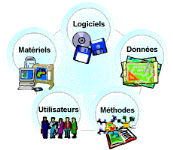
\includegraphics[width=0.25\textwidth]{img/cours/composants_sig.png}
	\caption{Les composants d'un SIG}
\end{figure}

La mise en oeuvre de ces deux composantes, organisationnelle principalement mais également technologique dans une moindre mesure, est intimement liée au domaine d'application du SIG : aménagement du territoire, gestion de réseaux, transport, télécommunication, géomarketing, recherche, etc.

Bien qu'adaptés à des contextes différents, les \textbf{logiciels SIG} ont en commun des fonctionnalités que l'on retrouve dans chaque système. Ces fonctionnalités sont couramment regroupées en cinq familles, "les 5A" :
\begin{itemize}
	\item \textbf{Abstraction}, pour rendre compte de la modélisation de la réalité;
	\item \textbf{Acquisition}, pour la collecte de données sous forme numérique;
	\item \textbf{Archivage}, pour le stockage des données dans un SGBD;
	\item \textbf{Affichage}, pour la représentation des informations;
	\item \textbf{Analyse}, pour la réalisation d'études
\end{itemize}

\begin{figure}[!h]
	\center 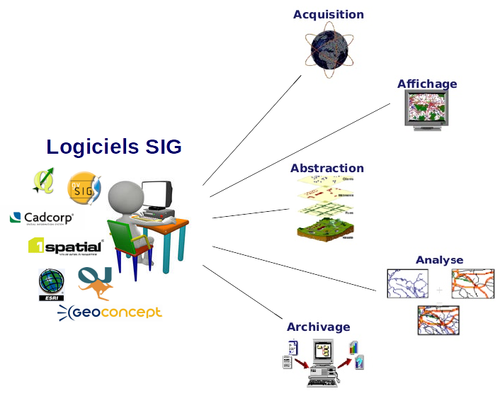
\includegraphics[width=0.55\textwidth]{img/cours/fonctionnalites_sig.png}
	\caption{Fonctionnalités d'un SIG : \textit{règle des 5A}}
\end{figure}

Chacune de ces fonctionnalités sera plus ou moins développée en fonction de la finalité du système d'information géographique dans l'organisation le mettant en place.

Les \textbf{données} sont dites \textbf{géographiques} lorsqu'elles sont associées à une information permettant de les localiser sur le terrain de manière explicite (coordonnées) ou implicite (adresse, nom de localité, etc.). Le géocodage est le processus permettant de transformer les références géographiques implicites et références explicites. On distingue par ailleurs deux types de représentation des données :
\begin{itemize}
	\item le modèle raster constitué d'une matrice de points, adapté aux phénomènes continus;
	\item le modèle vecteur où les informations sont regroupées sous la forme de coordonnées (points) ou successions de coordonnées (lignes, polygones), utile pour représenter les phénomèes discrets.
\end{itemize}

Si l'ordinateur de bureau a longtemps été le seul support des logiciels SIG, d'autres supports (ordinateurs portables, tablettes) permettent maintenant de traiter les données géographiques sur le terrain.

Enfin, les SIG mettent en oeuvre des ressources humaines variées (géomaticien, décideur, usager) qui vont permettre d'exploiter toute la richesse des logiciels.

La mise en oeuvre et l'exploitation d'un SIG ne peut s'envisager sans le respect de certaines règles et procédures propres à chaque organisation. 

\begin{center}
\fbox{
\begin{minipage}{.8\textwidth}
\paragraph{Bref historique des SIG}
\small \textit{La première application reconnue de l'analyse spatiale est datée de 1854 lorsque le docteur John Snow mène une étude sur la propagation d'une épidémie de choléra dans un quartier de Londres.
\\
Dans les années 1960 ensuite, alors que les cartes de l'époque étaient inadaptées, l'idée d'utiliser l'outil informatique pour déterminer les meilleurs lieux de plantation forestières en Afrique a fait sont apparition.
\\
Puis à partir des années 1970, les progrès importants des technologies informatiques ont contribué à accroître le développement des SIG.
4 grandes périodes (Maguire et al. 1991) :
\\
\begin{itemize}
	\item 1950 -1970 : premières applications de l'informatique à la cartographie;
	\item 1970- 1980 : les outils SIG font leur entrée dans les organismes étatiques (armée, cadastre, services topographiques, ...) ;
	\item 1980 -1990 : développement de plusieurs applications informatiques dédiées aux SIG et mise en réseaux des outils SIG;
	\item fin des années 1990 à nos jours : développement du webmapping avec plusieurs services cartographiques offerts sur internet et apparition de plusieurs outils libres ainsi que l'usage des technologies GPS.
\end{itemize}
}
\end{minipage}
}
\end{center}


\subsection{Serveurs SIG}

\subsubsection{Contexte}
L'utilisation dans de nombreuses branches métiers (assurance, transport, groupes pétroliers, etc.) de données présentant une composante géographique n'est pas nouveau : on estime qu'en 1980, 80\% des données stockées dans les bases de données avaient une composante spatiale implicite ou explicite \footnote{FRANKLIN K., \textit{An introduction to GIS: linking maps to databases}, 1992.}. Néanmoins, l'exploitation de la composante géographie est longtemps restée du seul ressort du géomaticien expert manipulant les solutions bureautiques décrites dans la partie précédente.

L'émergence des technologies connectés vers la fin du 20\up{ème} siècle a permis la diffusion de ces données auprès du grand public. Des initiatives comme Google Maps / Google Earth, en 2005, ont rendu possible la consultation de données géographiques par de larges communautés d'utilisateurs et ont largement démocratisé l'information géographique. 

Mais ces utilisateurs nouveaux n'ont pas besoin de toute la richesse du SIG, ni les compétences pour l'exploiter. Ils recherchent simplement des interfaces utilisateurs conviviales et robustes dédiées à des activités bien précises. Ces consommateurs peuvent être le grand public ou encore les différents corps de métier manipulant des données géo-référencées dans l'exercice de leurs missions. 

Il n'est donc plus question ici de SIG au sens propre du terme puisque ces nouvelles applications ne proposent pas systématiquement l'ensemble fonctionnalités au sens la règle des 5A. On parle d' \textbf{applications web SIG}.

La consommation d'informations géographiques par des utilisateurs séparés implique nécessairement que ces informations ait été mises à disposition par une tierce personne. Les solutions \textbf{serveurs SIG} répondent à cette problématique de partage des données. 

\begin{center}
\fbox{
\begin{minipage}{\textwidth}
La technologie \textbf{serveur SIG} est complémentaire de la technologie \textbf{bureautique}, en ce sens qu'elle permet de diffuser ce qui a été créé avec les outils bureautiques : les données géographiques, les cartes, les modèles d'analyse et de traitement.
\end{minipage}
}
\end{center}

Un serveur SIG répond à trois problématiques :
\begin{enumerate}
	\item \textbf{Héberger des ressources SIG} : le premier rôle d'un serveur SIG est bien d'héberger des ressources SIG qui seront consommées par les clients. On entend par ressource SIG les données géographiques et traitements sur ces données.
	\item \textbf{Publier des ressources SIG} : afin de rendre les ressources partageables, un serveur expose ses ressources sous forme de services. Un service peut être vu comme la représentation normalisée d'une ressource, rendue de ce fait consommable par différents clients sur un réseau ; le partage peut être limité à une entreprise (intranet, réseau local), étendu à un ensemble de partenaires (extranet, accès sécurisé par identifiant et mot de passe) voire étendu à tout l'internet.
	\item \textbf{Permettre d'interagir avec les ressources SIG} : il s'agit de permettre le déploiement d'applications web SIG qui consommeront les ressources publiées par le serveur sous forme de service. 
	Un service est destiné à être consommé par des applications de nature très différentes, développées dans des langages différents mais toutes capables d'interagir avec son interface normalisée (notion d'interopérabilité). Une telle interface s'appelle une API.
\end{enumerate}


\subsubsection{Environnement client/serveur}
L'environnement client/serveur désigne un mode de communication entre plusieurs programmes : l'un, qualifié de \textbf{client}, envoie des requêtes; l'autre, qualifié de \textbf{serveur}, attend les requêtes du client et y répond. Par extension, le client désigne l'ordinateur sur lequel est exécuté le logiciel client et le serveur l'ordinateur sur lequel est exécuté le logiciel serveur.

Il existe une grande variété de logiciels serveurs et clients répondant à des besoins spécifiques : serveur web, serveur de messagerie électronique, serveur de données, serveur cartographique, etc. Un serveur peut par ailleurs lui-même être le client d'un autre serveur et lui envoyer des requêtes. c'est par exemple le cas du serveur web qui fera appel à un serveur de cartographique pour afficher une carte dans un navigateur. L'architecture peut être découpée en autant d'étages (ie. de couple client/serveur) que nécessaires : on parle d'\textbf{architectures n-tiers}.

Cette organisation en couche présente l'avantage de pouvoir spécialiser chacune d'entre elles dans une tâche précise et de leur allouer des ressources adaptées en fonction de ces opérations à accomplir.

\begin{center}
\fbox{
\begin{minipage}{0.8\textwidth}
\small
\textit{Dans l'organisation client / serveur originel, le client envoie une requête au serveur qui effectue tous les traitements et retourne un résultat mis en forme. On parle de \textbf{client léger}.\\
A l'opposé, un \textbf{client lourd} support l'ensemble des traitements. Le serveur n'est, dans ce type de couple client-serveur, sollicité que pour mettre à disposition du client les données demandées.\\
Dans une architecture de type client riche, on tente de proposer un compromis pour optimiser les échanges avec le serveur. Une partie des traitements sont effectuées sur le serveur et un partie est effectuée par le client.}
\end{minipage}
}
\end{center}


\subsubsection{Architectures de serveurs SIG}
Ce qu'on appelle un serveur SIG est en fait une construction théorique reposant sur une architecture n-tiers qui sépare nettement ce qui touche à l'archivage des données, aux traitements métiers et au dialogue avec l'utilisateur. Derrière ce serveur théorique se cachent donc le plus souvent plusieurs machines physiques, chacune jouant un rôle bien précis : le serveur web chargé du dialogue HTTP, le serveur proxy qui masque les autres machines, les serveurs métiers et les serveurs de données.

Dans le cas le plus simple, l'ensemble des fonctionnalités serveur sont portées par une même machine.
\begin{figure}[H]
	\center 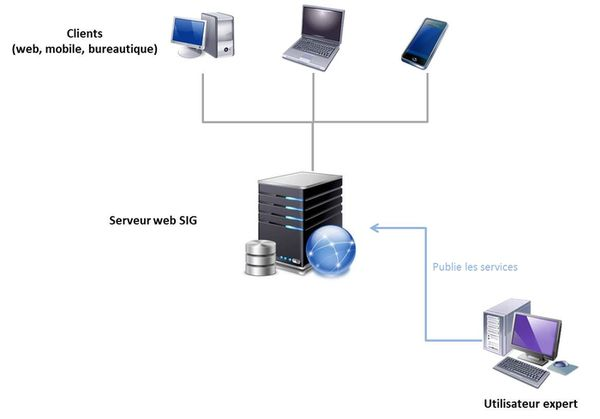
\includegraphics[width=0.65\textwidth]{img/cours/archi_serveur_sig-1.jpg}
	\caption{Serveur SIG en architecture 2-tiers}
\end{figure}

Une organisation plus courante consiste à séparer le serveur web du serveur cartographique.
\begin{figure}[H]
	\center 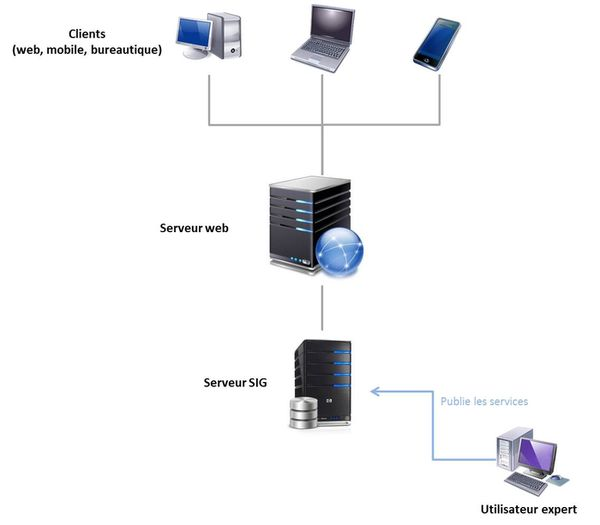
\includegraphics[width=0.65\textwidth]{img/cours/archi_serveur_sig-2.jpg}
	\caption{Serveur SIG en architecture 3-tiers}
\end{figure}

En poursuivant la logique de spécialisation des serveurs, la partie métier peut encore être séparée en deux : un serveur de données (ArcSDE, PostGIS, etc...) et un serveur SIG "pur" dédié aux géotraitements sur les données :
\begin{figure}[H]
	\center 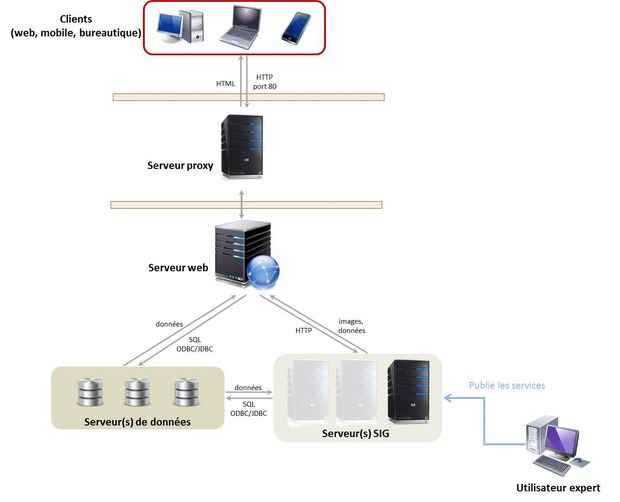
\includegraphics[width=0.7\textwidth]{img/cours/archi_serveur_sig-4.jpg}
	\caption{Serveur SIG en architecture 4-tiers}
\end{figure}

\begin{center}
\fbox{
\begin{minipage}{0.8\textwidth}
\small \textit{Les offres de données et de traitement totalement distribuées, le \textit{cloud computing}, se sont généralisées et permettent maintenant à un grand nombre d'utilisateurs d'accéder à des fonds cartographiques et à des outils SIG. Les géo-webservices se sont banalisés auprès du grand public et du monde de l'entreprise en quelques années seulement. Certaines offres sont gratuites d'autres commerciales. Dans les deux cas c'est une évolution de modèle économique importante puisqu'aujourd'hui il n'est plus toujours nécessaire d'acquérir des serveurs SIG ou de maintenir des bases de données géographiques référentielles. Une connexion web suffit pour bénéficier de la puissance des services géographiques.}
\end{minipage}
}
\end{center}


\newpage


\section{Les différents types de développement sous SIG}
La plupart des SIG proposent une interface de développement permettant de répondre à des besoins non couvert par les versions standards. Cette partie se propose de classifier les différents types de développement possibles sous SIG.


\subsection{Développements bureautiques}
\subsubsection{Personnalisation}
Face à des logiciels SIG souvent riches en fonctionnalités au point de les rendre parfois complexes, la première des demandes des utilisateurs est de pouvoir manipuler une interface adaptée à leur usage. 

En première approche, le géomaticien peut faire appel à des procédés "classiques" pour personnaliser des applications : ajouter/supprimer des barres d'outils, en créer de nouvelles en agrégeant des boutons. Cette approche reste néanmoins limité en terme de personnalisation.

Pour apporter plus de finesse dans la customisation de l'interface utilisateur, des interfaces de programmation sont disponibles sur certaines plateforme SIG. Elles permettrons par exemple de ré-agencer les cadres de la fenêtre ou de manipuler des barres d'outils ou menus jusque là inaccessibles.


\subsubsection{Automatisation de tâches répétitives}
Ce type de programmation concerne exclusivement le volet analyse des fonctionnalités des SIG (les "5A"). Le plus souvent à l'aide de scripts, le programmeur va pouvoir enchaîner plusieurs traitements que l'opérateur aurait eu à lancer manuellement.

En fonction des langages de scripts retenus par les éditeurs SIG, l'automatisation pourra être plus ou moins avancée et intégrer des structures conditionnelles et boucles pour faire varier les chaînes de traitements en fonction de l'état des données.


\subsubsection{Extension d'application existantes}
Cette partie de la programmation sous SIG comprend le développement de plug-ins venant étendre les fonctionnalités standards d'un SIG. Les développements pourront être plus lourds à mettre en place en fonction des technologies employées.


\subsubsection{Création d'application}
Dans cette rubrique, le programmeur va pouvoir concevoir en intégralité des applications se basant sur les fonctionnalités de base des SIG. L'éventail des possibilités dépendra de la manière dont les API exposent les fonctionnalités du SIG.
Notons toutefois que les applications développées de cette manière ne seront plus nécessairement des logiciels SIG au sens du respect de la règle des 5A (cas d'un simple visualiseur par exemple).



\subsection{Développements de solutions web}
Apparu dans les années 2000, les solutions web SIG font aujourd'hui parti du paysage informatique. Les éditeurs de SIG se sont adaptés à ce marché en proposant des solutions de conceptions d'applications cartographiques pour le web.

L'objectif de tels développement est de fournir aux utilisateurs finaux une application web SIG qui leur permette de travailler avec des données géographiques sans pour autant disposer de connaissances approfondies dans le domaine des SIG. L'apparente simplicité d'utilisation de certaines applications web SIG cache en réalité une analyse du besoin avancée et des développements parfois pointus qui visent à composer une application à partir : d'un fond de carte, d'une(de) couche(s) métier, d'outils et de bases de données géographiques.

\subsection{Développements de solutions mobiles}
Secteur en pleine extension, il s'agit de concevoir des applications nomades grand public fonctionnant sur les principaux OS du marché des smartphones.

Si les éditeurs de SIG proposent quasiment tous des solutions pour mobiles (smartphone, tablettes ou support spécifique), la liste de ceux permettant la conception ou personnalisation de tels applications est encore réduite.

La logique de conception d'une solution mobile est similaire à celle de conception d'une solution web : il s'agit de proposer une application métier simple d'usage pour un utilisateur final ayant peu de connaissance des SIG. 

%\subsection{Récapitulatif des solutions pour quelques SIG du marché}
%
%\begin{tabular}{|l|c|c|c|c|c|}
%	\hline
%	 & 
\includegraphics[width=0.05\textwidth]{img/cours/logo_esri.jpg} & 
\includegraphics[width=0.06\textwidth]{img/cours/logo_qgis.jpeg} & 
\includegraphics[width=0.1\textwidth]{img/cours/logo_geoconcept.jpg} & 
\includegraphics[width=0.06\textwidth]{img/cours/logo_mapinfo.jpg} & 
\includegraphics[width=0.06\textwidth]{img/cours/logo_openjump.jpeg} \\
%	\hline
%	\textbf{Personnalisation de l'interface} & X & X & X & X & X \\
%	\hline
%	\textbf{Automatisation de tâches} & X & X & X & X & X \\
%	\hline
%	\textbf{Extension d'applications} & X & X & X & X & X \\
%	\hline
%	\textbf{Création d'applications} & X & X &  & X &  \\
%	\hline
%	\textbf{Conception de solutions web} & X & X & X & X &  \\
%	\hline
%	\textbf{Conception de solution mobiles} & X &  & X &  &  \\
%	\hline
%\end{tabular}

\newpage



\section{Présentation du système ArcGIS}
ArcGIS est une suite intégrée d'applications logicielles de type SIG. Les différents produits donnent accès aux données géographiques dans un contexte  bureautique, à travers un réseau intranet ou internet ou encore depuis le terrain. L'ensemble forme un système complet de création, d'administration, d'exploitation, de communication et de diffusion d'informations géographiques (données ou services).

\begin{figure}[H]
	\center 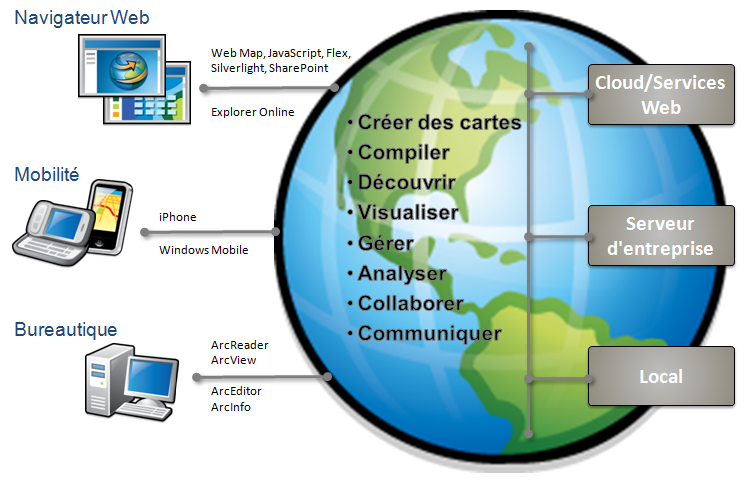
\includegraphics[width=0.6\textwidth]{img/cours/le_systeme_arcgis_10.png}
	\caption{Le système ArcGIS}
\end{figure}

ArcGIS s'adresse aux deux grandes catégories d'utilisateurs d'information géographique que sont les producteurs et les consommateurs. Les produits bureautiques à destination des producteurs (professionnels de l'information géographique) permettent essentiellement la modélisation des phénomènes, la collecte des données, les prétraitements et l'analyse. C'est le SIG au sens historique. Tandis que les applications web et mobiles fournies sur étagère ou développées ciblent davantage les consommateurs (ceux qui travaillent à partir d'une information déjà mise en forme et rendue intelligible). 

\begin{figure}[H]
	\center 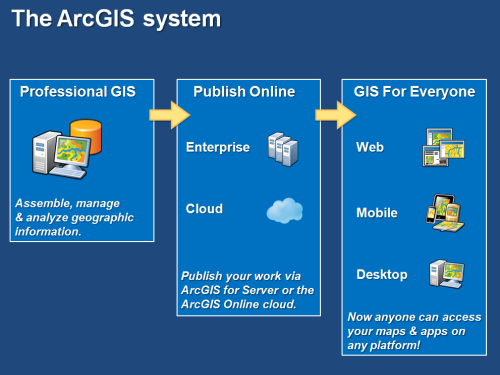
\includegraphics[width=0.6\textwidth]{img/cours/le_systeme_arcgis_10-2.png}
	\caption{Organisation du système ArcGIS}
\end{figure}

Enfin, aujourd'hui ArcGIS est par nature un SIG en ligne. Il faut comprendre par-là que chaque application ArcGIS peut fonctionner comme un client qui consomme de l'information géographique délocalisée sous forme de services. Et ce, qu'il s'agisse d'un client bureautique, web ou mobile. Autrefois exclusivement locales, les ressources sont de plus en plus disséminées sur les réseaux d'entreprises, voire sur le web pour celles qui ne sont pas confidentielles.


\subsection{Les applications bureautiques}
Il s'agit essentiellement d'ArcGIS for Desktop : une suite de logiciels Windows composée d'ArcMap, ArcCatalog, ArcGlobe, ArcScene et la nouvelle application ArcGIS Pro. Le produit inclus également les applications ArcToolbox et ModelBuilder. Il couvre l'ensemble des activités SIG : 
\begin{itemize}
	\item créer et mettre à jour de la donnée géographique;
	\item administrer des bases de données contenant de l'information géographique;
	\item intégrer des données existantes archivées dans divers formats;
	\item diffuser les données dans divers formats;
	\item créer des cartes ou des globes;
	\item prétraiter et analyser les données;
	\item créer des modèles de géotraitement.
\end{itemize}

\begin{figure}[!h]
	\center 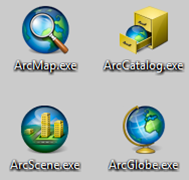
\includegraphics[width=0.25\textwidth]{img/cours/arcgis_for_desktop.png}
	\caption{Applications traditionnelles d'ArcGIS for Desktop}
\end{figure}

Sortie avec la version 10.3 d'ArcGIS for Desktop, ArcGIS Pro est le dernier né des outils Esri. L'ergonomie de l'application y a été complètement repensée en intégrant notamment le ruban en haut de l'application (à la manière des applications du pack Office). Elle est conçu pour gérer des projets SIG dans leur intégralité : collecte, gestion, maintenance, analyse et cartographie de données géographiques. Elle rend par ailleurs possible l'exploitation de données 2D et 3D dans le même logiciel.

\begin{figure}[!h]
	\center 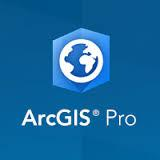
\includegraphics[width=0.15\textwidth]{img/cours/arcgis_pro.jpg}
	\caption{Application ArcGIS Pro}
\end{figure}

L'ensemble de la suite est fournie sous trois niveaux de licence qui donnent accès à plus ou moins d'outils :
\begin{itemize}
	\item ArcView, pour l'utilisation, la cartographie et l'analyse des données ; 
	\item ArcEditor, qui ajoute les fonctions d'administration des géodatabases ;
	\item ArcInfo, qui offre un bureau SIG professionnel complet.
\end{itemize} 

Il s'agit d'un produit clé en main, qui peut toutefois être complètement adapté aux besoins de l'utilisateur. Des extensions pour le placement de toponymes, l'analyse de réseaux ou encore le géomarketing viennent également compléter les fonctionnalités du noyau SIG.

\begin{center}
\fbox{
\begin{minipage}{\textwidth}
ArcGIS Desktop occupe, au sein de l'organisation mettant en place un SIG, une place tout à fait centrale. C'est lui qui permet de créer les ressources qui pourront ensuite être partagées en interne ou sur le web.
\end{minipage}
}
\end{center}

On trouve également dans la famille des applications bureautiques ArcGIS Explorer, une application que l'on peut télécharger gratuitement et qui permet de visualiser des données géographiques mais aussi, dans une certaine mesure, de les exploiter. On peut notamment créer des cartes mêlant des sources de données diverses (locales, services web), utiliser quelques outils simples d'analyse spatiale (recherche sur critère de proximité).

Enfin les produits développés avec ArcGIS Engine se situent également dans la familles des applications bureautiques. ArcGIS Engine, c'est un ensemble d'outils conçu par Esri pour aider le développeur à créer d'applications bureautiques personnalisées intégrant des fonctions SIG.


\subsection{Les applications serveur}
ArcGIS propose deux produits serveurs : \textbf{ArcGIS for Server} et \textbf{ArcIMS}. Le premier remplacé le second qui n'est maintenu aujourd'hui que par soucis d'assurer la continuité du service vis-à-vis des clients historiques. 

ArcGIS for Serveur est constitué d'un ensemble d'outils et de technologies web permettant le partage de ressources SIG sur un réseau. Il s'agit d'un serveur SIG à part entière, c'est-à-dire d'un outil permettant d'interagir pleinement avec l'information géographique et notamment à des fins opérationnelles ou d'analyse. Une solution ArcGIS for Server peut être déployée sur des serveurs classiques ou dans le cloud à l'aide Amazon EC2 ou Microsoft Azur. Elle s'exécute dans des environnements Windows et Linux.

Tout comme la solution ArcGIS for Desktop, ArcGIS for Server est disponible en trois niveaux de licence (Basic, Standard et Advanced), qui se distinguent par leurs capacités de publication de services. 

Comme toutes les solutions web, une solution ArcGIS for Server s'inscrit avant tout dans une architecture client-serveur. 
\begin{figure}[H]
	\center 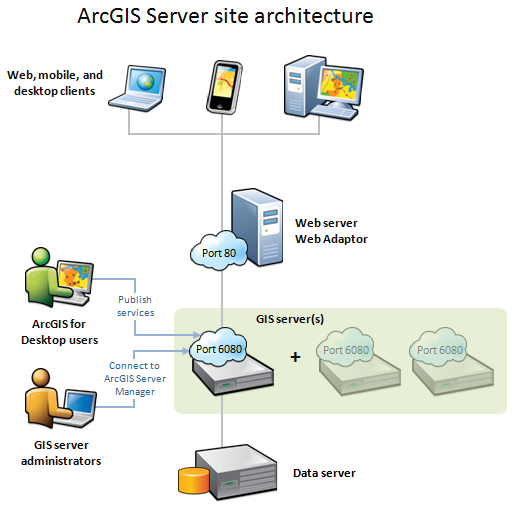
\includegraphics[width=0.7\textwidth]{img/cours/AcrGIS_Server_architecture.png}
	\caption{Architecture ArcGIS for Server}
\end{figure}
\vspace{2em}

\textbf{\emph{ArcGIS for Server permet d'héberger des ressources SIG}}, lesquelles sont de différentes  natures : 
\begin{itemize}
	\item des données vectorielles ou images (fichiers de forme, géodatabase) ;
	\item des données cartographiées (documents cartographiques, globes 3D) ;
	\item des géo-traitements ou fonctions permettant d'interagir et donc d'exploiter les données (ArcToolBox) ;
	\item des géo-traitements personnalisés, i.e. des chaînes de traitements SIG capable de produire de nouvelles informations à partir de données en entrée (ModelBuilder, scripts Python).
\end{itemize}

Pour permettre l'accès concurrent en édition aux données spatiales, il est nécessaire de les stocker dans une géodatabase d'entreprise. Ce type de géodatabase reprend le modèle de géodatabase classique en y ajoutant la gestion des accès multi-utilisateurs aux données. Ces géodatabases appelées aussi géodatabases ArcSDE sont prises en charge par plusieurs SGBD (Oracle, SQL Server, DB2, PostGreSQL, etc.). La mise en place d'une telle géodatabase suppose donc d'installer sur un serveur non seulement le serveur SIG mais aussi le SGBD. Depuis la version 9 d'ArcGIS, ArcSDE fait partie intégrante d'ArcGIS for Server. A noter que s'il ne s'agit que de fournir un accès web en consultation, les données peuvent être stockées sous forme de géodatabase personnelle ou fichier.
\vspace{2em}

\textbf{\emph{ArcGIS for Server présente ses ressources sous forme de services.}} Parmis les services les plus courant citons par exemple ceux de type cartographique, d'imagerie, de géotraitement, de géocodage, de globe ou encore d'analyse de réseau.

Les services d'ArcGIS for Server sont accessibles dans les applications bureautiques, mobiles et sur des navigateurs. Ils peuvent être combinés à des services web publics tels qu'OpenStreetMap ou World Topographic Map.

Pour publier un \textit{service de carte}, il faut d'abord créer une carte, i.e. un document ArcMap (mxd). Il faut ensuite le stocker dans un répertoire accessible par ArcGIS for Server et s'assurer que les données géographiques qu'il contient sont également accessibles par ArcGIS for Server.
Les feature services sont une évolution majeure de la version 10. Ils permettent à un client web HTTP d'accéder en lecture et en écriture aux objets géographiques.

Pour publier un \textit{service de géotraitement}, il y a 2 façons de procéder : soit on publie la toolbox,  soit on l'insère dans un document ArcMap et on publie le document. Il y a une différence à l'exécution du service : dans le premier cas, celui-ci doit faire des accès disque pour utiliser les données, tandis que dans le second il suffit de faire des accès mémoire. Si le géotraitement est coûteux en temps d'exécution, on privilégiera donc la deuxième solution. Il est possible aussi d'associer un geoprocessing service à un result map service. Par défaut, les données renvoyées par le service de géotraitement sont non symbolisées, elles sont livrées en vecteur au client: charge à lui de les symboliser. Le recours à un result map service permet au serveur de cartographier le résultat du géotraitement : le client n'a plus qu'à afficher l'image fournie.

Pour publier un \textit{service de géocodage}, il faut créer au préalable un locator ou localisateur d'adresses avec ArcCatalog. Un tel objet permet de décrire une méthode de géocodage (ex : géocodage à l'adresse postale) par rapport à un référentiel (ex : la BD Adresse® de l'IGN).

Les \textit{service de géodonnées} permettent d'interagir avec les données d'une geodatabase par le biais d'ArcGIS for Server. Ils permettent l'exploitation (requêtes) et l'administration (extraction, réplication…) de données à distance par le réseau. Là encore il y a deux façons de procéder : soit on publie directement une geodatabase, soit on ajoute à un document ArcMap les tables que l'on souhaite exposer et on publie le document.

\begin{table}[H]
	\begin{center}
		{\renewcommand{\arraystretch}{1.3}
		\begin{tabular}{|l|p{7 cm}|}
			\hline 
			\textbf{Type de service} & \textbf{Ressource SIG requise} \\
			\hline
			Service de carte & Document ArcMap (.mxd) ou définition de service de carte (.msd) \\
			Service de géocodage & Localisateur d'adresses (.loc, .mxs) \\
			Service de géodonnées & Géodatabase fichier ou fichier de connexion à une base de données (.sde) \\
			Service GeoEvent & Composants du service GeoEvent \\
			Service de géotraitement & Résultat du géotraitement de la fenêtre résultat dans ArcMap \\
			Service de globe & Document ArcGlobe (.3dd) \\
			Service d'imagerie & Jeu de données raster, mosaique ou fichier de couche faisant référence à un jeu de données raster ou mosaique \\
			Service de recherche & Dossiers et géodatabases de contenu SIG dans lesquelles effectuer  la recherche \\
			Service Workflow Manager & Référentiel ArcGIS Workflow Manager \\
			\hline
		\end{tabular}
	}
	\end{center}
	\caption{Services disponibles avec ArcGIS for Server}
\end{table}

Un \textit{service de géométrie} est par ailleurs créé automatiquement à l'installation d'ArcGIS for Server. Il ne peut y avoir qu'un seul service de géométrie. Il doit s'appeler \textit{Geometry}. Il s'agit d'une alternatives possible à certains services de géotraitements pour des opérations simples : buffer, simplification de polyligne, changement de système de coordonnées, etc. 

La publication d'un service ArcGIS for Server ne suffit pas à rendre la ressource pleinement exploitable par l'utilisateur. Il convient d'activer les \textbf{fonctionnalités} qui définissent la manière d'utiliser ce service. C'est l'activation de fonctionnalités qui permet de fournir la fonction SIG dont les utilisateurs auront besoin.

Par exemple, l'activation de la fonctionnalité \textit{Feature Access} d'un service de carte (document mxd publié) donnera à l'utilisateur la possibilité de manipuler les entités (requêtes, mise à jour, etc.). Notons que cela suppose que les données soient stockées dans une géodatabase ArcSDE autorisant l'édition multi-utilisateurs. D'un point de vue utilisateur, cela revient à manipuler un \textit{service d'entités}.

\begin{figure}[H]
	\center 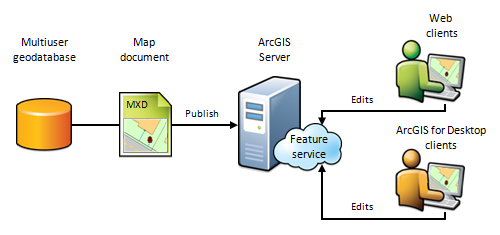
\includegraphics[width=0.65\textwidth]{img/cours/publication_feature_service.png}
	\caption{Création d'un \textit{service d'entités}}
\end{figure}

On administre les services (création, arrêt, démarrage, paramétrage) à l'aide  d'ArcCatalog ou d'une application web, livrée avec ArcGIS for Server, le \textbf{Manager}. Il est également possible de publier certains services depuis ArcGIS Online (cf. paragraphe suivant).

\begin{table}[H]
	\begin{center}
		\footnotesize
		\begin{tabular}{|m{3 cm}|p{7 cm}|p{3 cm}|}
			\hline 
			\textbf{Fonctionnalité} & \textbf{Utilité} & \textbf{Services présentant cette fonctionnalité} \\
			\hline
			Accès aux données & Permet d'accéder aux entités vectorielles d'une carte. & Service de carte \\
			Géocodage & Permet d'accéder à un localisateur d'adresses. Cette fonctionnalité est toujours activée lors de la publication d'un service de géocodage. & Service de géocodage \\
			Géodonnées & Permet d'accéder au contenu d'une géodatabase pour les requêtes, l'extraction et la réplication de données. Toujours activée pour un service de géodonnées. & Service de géodonnées \\
			Géotraitement & Permet d'accéder aux modèles de géotraitement. Toujours activée pour un service de géotraitement. & Service de géotraitement \\
			Globe & Permet d'accéder au contenu d'un document ArcGlobe. Toujours activée pour un service de globe. & Service de globe \\
			Traitement d'images & Permet d'accéder au contenu d'un jeu de données raster ou en mosaïque, y compris les valeurs de pixel, les propriétés, les métadonnées et les canaux. Toujours activée pour un service d'imagerie. & Service d'imagerie\\
			JPIP & Fournit les fonctionnalités JPIP de transmission en continu lors de l'utilisation de fichiers JPEG2000 ou NITF et lorsque la configuration est effectuée avec un serveur JPIP. & Service d'imagerie \\
			KML & Utilise une carte pour créer des entités KML. & Service d'imagerie \\
			Cartographie & Permet d'accéder au contenu d'une carte, tel que les couches et leurs attributs sous-jacents. Toujours activée pour un service de carte. & Service de carte \\
			Accès mobile aux données & Permet d'extraire des données d'une carte vers un périphérique mobile. & Service de carte \\
			Analyse de réseau & Permet de résoudre des problèmes liés à l'analyse de réseaux de transport à l'aide de l'extension ArcGIS Network Analyst. & Service de carte \\
			Schématics & Permet l'affichage, la génération, la mise à jour et la modification de diagrammes schématiques. & Service de carte \\
			WCS & Crée un service conforme à la spécification WCS (Web Coverage Service) émise par l'OGC (Open Geospatial Consortium, Inc.). & Service de carte, service d'imagerie, service de géodonnées \\
			WFS & Crée un service conforme à la spécification WFS (Web Feature Service) émise par l'OGC. & Service de carte, service de géodonnées \\
			WMS & Crée un service conforme à la spécification WMS (Web Map Service) émise par l'OGC. & Service de carte, service d'imagerie \\
			WMTS & Crée un service conforme à la spécification WMTS (Web Map Tile Service) émise par l'OGC. & Service de carte, service d'imagerie \\
			WPS & Crée un service conforme à la spécification WPS (Web Processing Service) émise par l'OGC. &Service de géotraitement  \\
			\hline
		\end{tabular}
	\end{center}
	\caption{Fonctionnalités activables par type de service ArcGIS for Server} 
\end{table}
\newpage

Et enfin, \textbf{\emph{ArcGIS for Server expose ses services à travers quatre APIs.}}

L'\textbf{API REST pour ArcGIS for Server} : c'est une interface très simple d'emploi qui expose les ressources sous forme d'URLs ; elle est donc utilisable par de simples clients HTTP capables d'envoyer au serveur des requêtes GET.

\begin{figure}[H]
	\center 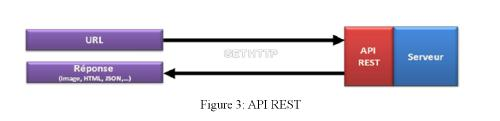
\includegraphics[width=0.80\textwidth]{img/cours/api_rest.jpg}
	\caption{Principe du protocole REST}
\end{figure}

L'\textbf{API SOAP pour ArcGIS for Server} : c'est une interface qui utilise HTTP et le langage XML pour permettre le dialogue entre le client et le serveur. Pour être tout à fait exact, cette API utilise les spécifications WSDL et SOAP du W3C. WSDL (Web Service Description Language) permet au fournisseur du service de décrire en XML la syntaxe des requêtes à lui adresser. SOAP est un protocole XML, i.e. un langage bâti sur XML pour permettre l'échange de messages client-serveur sur un réseau et notamment sur HTTP. Son emploi est moins direct que REST puisqu'il faut mettre en place et côté client et côté serveur des objets capables de générer et de parser les messages SOAP.

\begin{figure}[H]
	\center 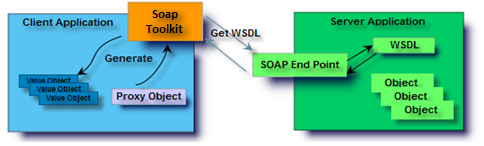
\includegraphics[width=0.70\textwidth]{img/cours/api_soap.png}
	\caption{Principe du protocole SOAP}
\end{figure}

Les \textbf{APIs OGC (WMS, WFS, WMC)} : l'OGC (Open Geospatial Consortium) édite des normes pour permettre l'échange de cartes et de données entre le plus grand nombre de système. ArcGIS for Server permet de publier trois types de services OGC : WMS (Web Map Services) pour fournir au format image les données de plusieurs couches, WFS (Web Feature Service) pour fournir au format GML des données vectorielles et WCS (Web Coverage Service) pour fournir au format grille des données raster. Ces services sont consommables par des clients OGC, et donc notamment des clients externes à la gamme ArcGIS (SIG QGIS, MapInfo, Géoconcept, API web comme OpenLayers ou Géoportail).

\textbf{KML} : c'est le format propriétaire Google pour échanger de l'information géographique. Il s'agit d'un langage XML utilisable avec les applications Google (Google Maps, Google Earth) mais également un standard de fait accepté en entrée par de nombreux systèmes.

Notons pour finir sur la partie exposition des ressources qu'Esri propose également une solution, \textbf{Portal for ArcGIS}, permettant de faciliter et de sécuriser la gestion de contenus dans une infrastructure. Cette extention d'ArcGIS for Server fournit un moyen de rendre les données SIG accessibles au non expert. Dans l'architecture d'un serveur SIG, elle va venir créer une couche supplémentaire s'intercalant entre le serveur SIG proprement dit et le consommateur de services SIG.

\begin{figure}[H]
	\center 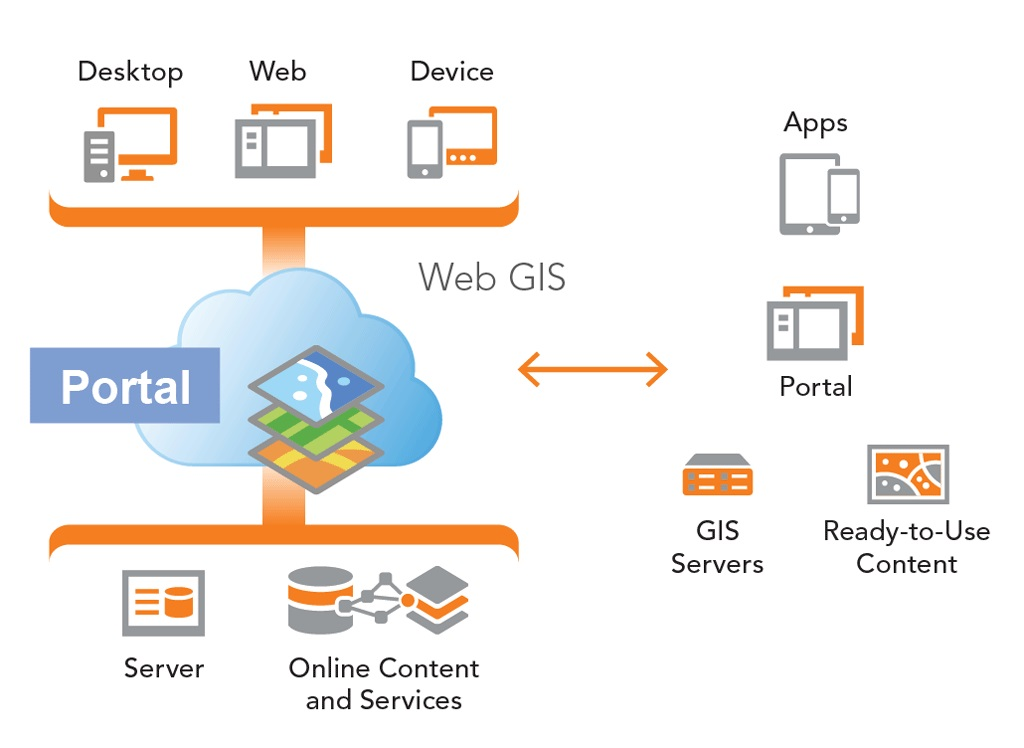
\includegraphics[width=0.55\textwidth]{img/cours/portal_for_arcgis.jpg}
	\caption{Architecture Portal for ArcGIS}
\end{figure}

Pour la conception d'applications web SIG, Esri proposes plusieurs solutions. La solution retenue dépendra des besoins de l'application et des compétences du concepteur : il pourra s'agir d'applications configurables à partir de modèles ou d'application web créées de entièrement à partir d'API. En focntion de la solution retenue, elle reposera sur l'une des trois technologies suivantes : Javascript, Flex ou Silverlight. En arrière plan, toutes ces solutions font appel à l'API REST d'ArcGIS pour consommer les services publiés.


\subsection{Services web hébergés - Le SIG dans le cloud}
Esri s'est adapté à la demande du marché de disposer de ressources SIG (cartes, données, traitements) facilement accessibles et consommable depuis n'importe quelle plateforme (bureautique, web, mobile). En s'appuyant sur sa technologie ArcGIS for Server, Esri propose une offre de service dans le cloud : \textbf{ArcGIS Online} (\textit{www.arcgis.com}).

\begin{figure}[H]
	\center 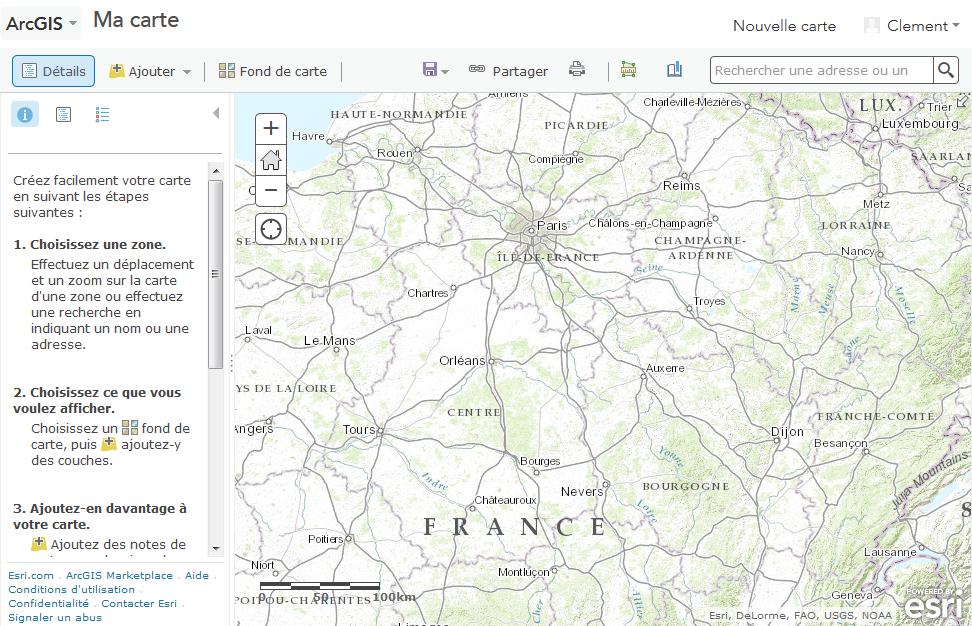
\includegraphics[width=0.7\textwidth]{img/cours/arcgis_online.png} 
	\caption{ArcGIS Online}
\end{figure}

Initialement limitée au partage de cartes, ArcGIS Online a vu ses fonctionnalités s'étoffer rapidement : possibilité d'ajouter ses propres données, effectuer quelques traitements simples sur celles-ci, créer de nouvelles cartes, de les partager sur le web, etc. C'est aujourd'hui l'offre de SIG dans le cloud la plus complète du marché.

Elle est proposée en plusieurs niveaux de licences qui donnent accès à plus ou moins de fonctionnalités. La version gratuite permet déjà de créer une application web SIG complète : choix d'un fond de carte, ajout de données métiers, utilisation de geo-traîtements simples. Il suffit de s'inscrire sur la plateforme pour pouvoir disposer de ce services. Les niveaux de licence les plus élevés permettent à l'organisation de disposer d'un serveur SIG complet hébergé sur les serveurs d'Esri. De nombreuses organisations font ce choix qui leur offre un serveur SIG sans avoir besoin de compétences de SIGiste.


\subsection{Les applications mobiles}
Cette catégorie d'applications regroupe des outils destinés à la fois aux professionnels mais aussi au grand public. Les professionnels ciblés sont amenés à  créer, mettre à jour, afficher et éventuellement analyser des données géographiques sur le terrain; le grand public lui est essentiellement consommateur d'information géographique ; certaines applications lui permettent néanmoins de contribuer à destination d'une communauté d'utilisateurs.

Le SIG mobile est toujours associé à un GPS chargé du recueil de la position et souvent à un certain nombre d'autres capteurs (boussole, accéléromètre, gyroscope…). Il est actuellement en plein essor et bénéficie de la maturité des technologies de positionnement GPS/GNSS et de télécommunication.

Leur valeur ajoutée pour l'entreprise est très grande : ils permettent aux gens des métiers (policiers, agents de réseau, urgentistes, scientifique, etc.) d'alimenter eux-mêmes le système d'information.

Esri propose trois types d'applications mobiles SIG : 
\textbf{ArcPad} qui est une application sur étagère que l'on peut personnaliser avec l'environnement ArcPad Application Builder. ArcPad s'installe sur chacun des périphériques à équiper. Il est possible d'interfacer ArcPad avec une solution ArcGIS Server, permettant ainsi aux équipes de terrain de travailler en direct ou en déconnecté avec les données hébergées par le serveur. La mise en œuvre d'une telle solution nécessite de publier les données à mettre à jour sur le terrain sous forme d'un service de carte (document Arcmap) compatible pour un usage dans ArcPad. La création d'un tel service nécessite l'ajout de l'extension ArcPad pour ArcGIS Server. La mise à jour de données par des équipes de terrain suppose également un accès concurrentiel à une même source de données, donc un stockage SGBD dans une geodatabase ArcSDE.
\begin{figure}[H]
	\center 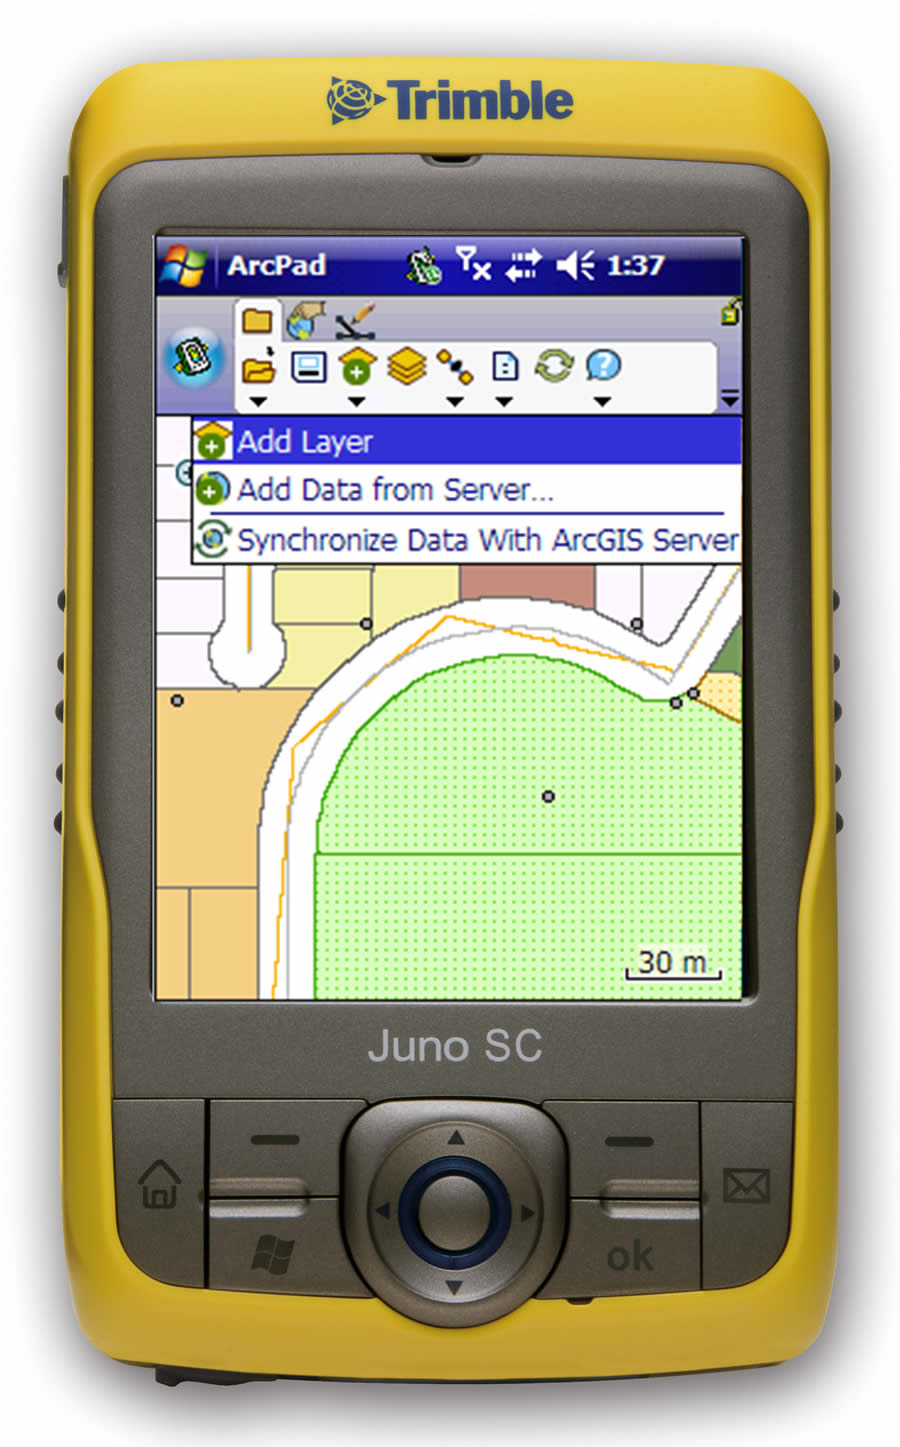
\includegraphics[width=0.15\textwidth]{img/cours/arcpad.jpg}
	\caption{Périphérique ArcPad}
\end{figure}
	
\textbf{ArcGIS Mobile} qui est à la fois une application et un kit de développement permettant de déployer des clients mobiles autonomes ou bien légers communiquant via des réseaux sans fil avec un serveur ArcGIS.
\begin{figure}[H]
	\center 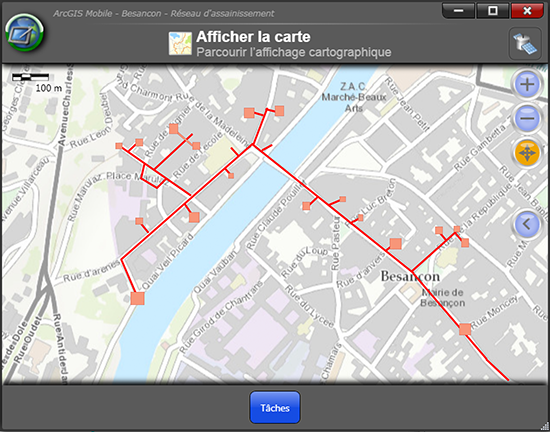
\includegraphics[width=0.47\textwidth]{img/cours/arcgis_mobile.png}
	\caption{Exemple d'application ArcGIS Mobile}
\end{figure}

\textbf{ArcGIS pour smartphones} qui est en fait un ensemble d'applications et d'APIs natives pour les principaux OS de téléphonie mobile : Windows Phone, IPhone et Androïd. 

\begin{figure}[H]
	\center 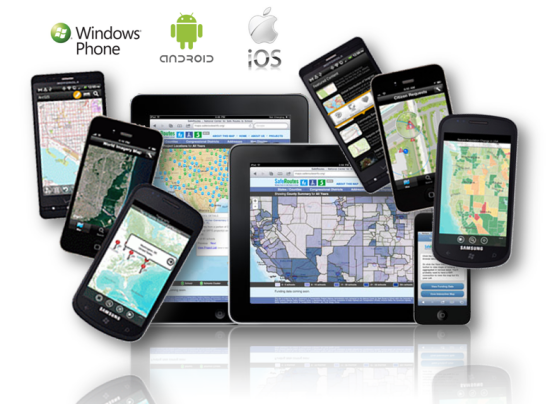
\includegraphics[width=0.6\textwidth]{img/cours/arcgis_for_smartphone.png}
	\caption{Exemples d'applications ArcGIS pour smartphone}
\end{figure}

Les trois types d'applications ont la capacité à consommer les services hébergés par les serveurs Esri (ArcGIS Online) ce qui permet aux organisations de se focaliser sur les données métier.

Depuis peu, Esri propose également une solution métier pour smartphone prête à l'emploi : \textbf{Collector for ArcGIS}. Fonctionnant actuellement sur Android ou iOS, cette application est destinée à la saisie ou mise à jour d'information directement sur le terrain. Elle est prévu pour pouvoir continuer à travailler même sans connexion et peut attaquer des données d'ArcGIS Online ou d'un serveur SIG traditionnel. On remarquera que ce type d'application contribue à gommer un peu plus la frontière entre producteur expert et consommateur de ressources SIG puisqu'elle permet à tout un chacun de saisir dans des bases partagées de l'information géographique.

\begin{figure}[H]
	\center 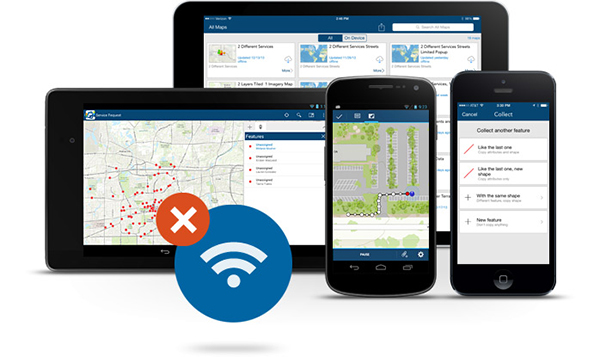
\includegraphics[width=0.6\textwidth]{img/cours/collector_for_arcgis.jpg}
	\caption{Application Collector for ArcGIS}
\end{figure}

\newpage



\section{Développements sous la plate-forme ArcGIS}

\subsection{Panorama des différentes APIs}
La plate-forme ArcGIS offre de multiples possibilités de développement. Elle permet de couvrir les besoins habituels sous SIG de développement de : scripts, extensions, applications métiers, applications web, applications mobiles.

De manière cohérente avec les tendances affirmées en faveur du web SIG, ArcGIS est particulièrement adapté au développement de web application SIG, i.e. d'application orientée métier, dotée d'une ergonomie proche de celle d'une application bureautique et exécutable dans un simple navigateur web.

Récemment, ArcGIS s'est également ouvert largement au développement d'application nomade grand public, i.e. d'application native pour les principaux OS du marché des téléphones intelligents (iOS, Androïd, Windows Phone).

D'une manière générale, les fonctionnalités du SIG sont rendues accessibles pour le développeur à travers des interfaces de programmation (API) et des kits de développement logiciel (SDK).

On distinguera 4 grandes familles d'APIs :
\begin{itemize}
	\item l'API Python;
	\item l'API ArcObjects et les SDK Runtime;
	\item les API web;
	\item les API mobiles.
\end{itemize}

La force d'ArcGIS tient en grande partie à sa large communauté d'utilisateurs. Cette communauté représente une aide précieuse pour le développeur novice ou chevronné, et ce notamment à travers les nombreux codes source présents sur le web qui s'ajoutent à la documentation très riche qui accompagne chacun des SDK. A l'heure actuelle, toute l'information utile est mise à disposition sur le centre de ressources ArcGIS (\textit{http://resources.arcgis.com}).


\subsection{L'API ArcObjects}
L'\textbf{API ArcObjects} est l'API fondamentale d'ArcGIS. Elle expose les fonctionnalités à un niveau de détail très fin. C'est elle qui offre la plus grande souplesse pour le développement d'extensions ou bien d'applications dans un contexte bureautique.

ArcGIS est une plate-forme logicielle conçue comme un ensemble de composants. Par composants, on entend des briques réutilisables pour le développement d'applications tierces et ce quel que soit le langage utilisé. Un composant logiciel se présente donc au format binaire et non sous forme de code source. Il est indépendant des applications qui l'utilisent. Une dll ou un control ActivX sont des exemples de composants logiciels.

Cela  étant, pour déployer des composants il faut non seulement les compiler pour produire le code binaire mais aussi créer des interfaces afin d'exposer leurs fonctionnalités de manière exploitable par des applications clientes. Afin d'être comprises par tout programme, ces interfaces doivent être standardisées : elles doivent suivre une norme. Le développement logiciel à base de composants est donc un développement en couche distinguant très clairement les traitements de leur présentation au monde extérieur. Pour les traitements on parle de \textbf{classes métiers} (ou business objects) ; pour la couche présentation on parle d'\textbf{interfaces}. Les classes métiers implémentent des interfaces qui elles seules permettent le dialogue entre le client consommateur et le serveur qui exécute le traitement demandé. Ces concepts sont directement tirés du mode de pensée orientée-objet dont l'un des grands principes est l'\textbf{encapsulation}. Ils ont profondément modifié l'industrie du développement logiciel depuis leur apparition au début des années 90 et sont aujourd'hui complètement généralisés, notamment au travers des architectures à base de web services. Un web service n'est autre en effet qu'un programme interrogeable par un autre programme par le biais d'une interface normalisée.

Les ArcObjects sont les composants d'ArcGIS, développés en C++, et rendus consommables à travers des interfaces \textbf{COM} (Component Object Model). COM est un standard introduit par Microsoft en 1995 favorisant le développement d'une application sous forme de composants autonomes et réutilisables, quel que soit le langage dans lequel elle est codée (COM impose l'usage d'un langage normalisé, l'IDL, pour décrire les interfaces des objets). D'autres technologies sont apparues depuis apportant des réponses aux nouveaux besoins suscités par les architectures client-serveur et distribuées (généralisation de l'emploi de composants distants). Les composants COM sont toutefois compatibles avec ces technologies et aujourd'hui ArcGIS 10 qui s'exécute en environnement .Net 3.5 les utilise toujours.

Pour écrire du code faisant appel aux fonctionnalités du SIG, le développeur utilisant les ArcObjects manipule donc un ensemble d'interfaces (COM, .Net). Une interface dans la terminologie des langages orientés-objet est une \textbf{classe virtuelle}, c'est à dire une classe dont les membres sont des \textbf{méthodes virtuelles} (ie. déclarée mais non définie dans la classe). Les classes métiers quant à elles implémentent les méthodes virtuelles d'une ou plusieurs interfaces.

La réunion de toutes ces interfaces se nomme en fait une \textbf{API} (Application Programming Interface). L'API ArcObjects contient de nombreuses interfaces lesquelles sont fort heureusement très bien documentées, notamment à l'aide de diagramme de classe UML installés avec le logiciel.

\begin{figure}[!h]
	\center 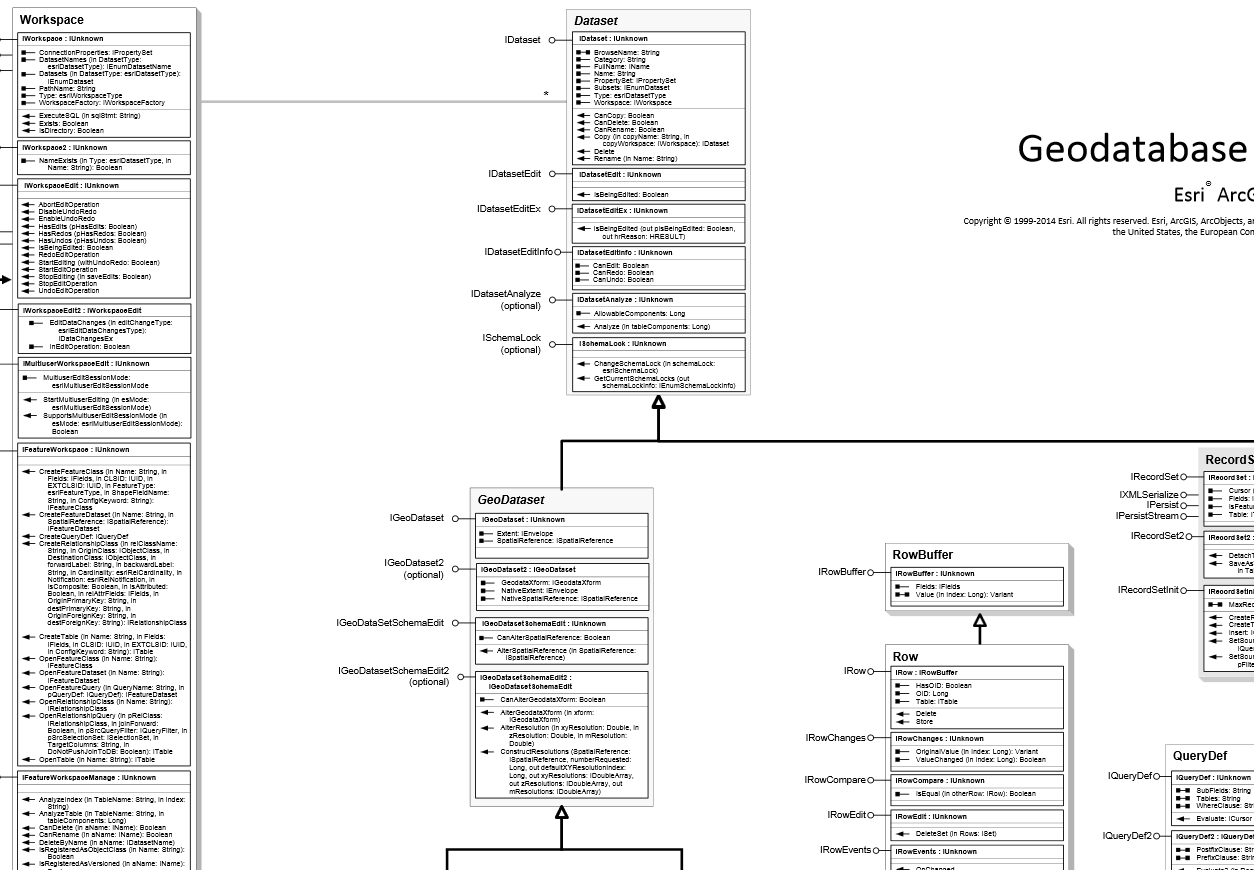
\includegraphics[width=0.70\textwidth]{img/cours/api_arcobjects.png}
	\caption{Exemple de diagramme ArcObjects}
\end{figure}

Le développeur a comme on l'a vu dans les paragraphes précédents une liberté quant au choix du langage de programmation pour utiliser cette API. Esri l'aiguille tout de même en proposant des \textbf{SDK} (kit de développement) qui permettent de construire facilement des applications se basant sur l'API ArcObject.

Le SDK .Net permet de développer des extensions pour ArcGIS for Desktop dans un environnement .Net : on parlera de \textbf{SDK ArcObjects for .Net}. Ces extensions peuvent prendre la forme d'add-ins facilement déployables sur un parc informatique. Ces add-ins permettent d'ajouter des éléments personnalisés à l'interface graphique des applications. Au-delà, le SDK permet également d'étendre les fonctionnalités des classes métiers (les ArcObjects) tant des versions bureautique que serveur, mais aussi de créer de nouvelles applications à dimension spatiale. Pour l'utiliser il faut disposer de l'IDE Microsoft Visual Studio (la version Express peut suffire) et connaître un des langages VB.Net ou C\#.Net, voir ASP.Net pour les développements serveur.

Le \textbf{SDK ArcObject for Java} propose les mêmes fonctionnalités que le SDK ArcObjects for .Net à la différence qu'il permet de créer des applications exécutables dans n'importe quel système d'exploitation. Ce SDK s'intègre à l'IDE Eclipse. Il faut bien entendu utiliser ici le langage Java pour coder.

Jusqu'à la version 10.0 d'ArcGIS, un environnement de développement VBA, qui est un environnement COM natif, était intégré à ArcGIS et utilisait directement l'API ArcObjects. Ce langage a été remplacé dans l'environnement ArcGIS, par Python qui peut également manipuler directement les composants COM. Les SDK .Net et Java sont toutefois préconisé pour les développements faisant appel aux ArcObjects. 
les bibliothèques étaient utilisées de manière directe par le SDK VBA qui est un environnement COM natif

\textbf{\emph{Remarque : composants in- et out-of-process}}

Les composants peuvent être rangés dans deux grandes catégories : les composants \textit{in-process} et les composants \textit{out-of-process}. Les in-process sont exécuté dans le même processus que l'application qui les utilise. Les out-of-process sont exécutés dans les processus séparés. Pour cette dernière catégorie, on distingue les composants locaux qui s'exécutent sur la même machine que l'application client des composants distants qui s'exécute sur une autre machine reliée par le réseau.

Lorsque l'on installe ArcGIS sur une machine, parmi tous les fichiers copiés sur le disque on trouve les composants binaires et leurs interfaces. Les composants binaires sont stockés dans le sous-dossier bin du répertoire d'installation, tandis que les interfaces sont dans le sous-dossier com.
On constate que le dossier bin contient à la fois des composants de type in-process (\textbf{.dll}, \textbf{.ocx}) et des composants de type out-of-process (\textbf{.exe}).

\begin{figure}[H]
	\center 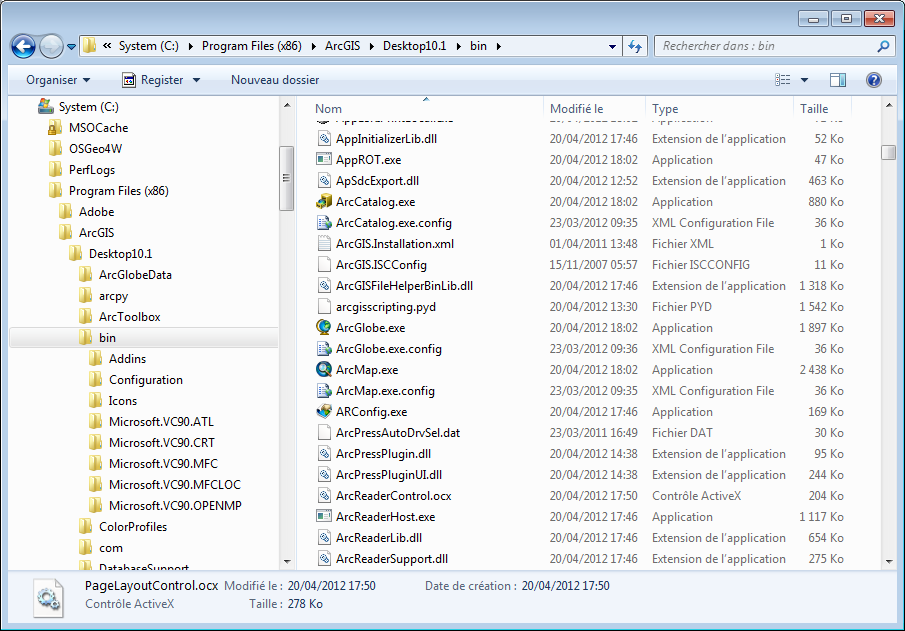
\includegraphics[width=0.70\textwidth]{img/cours/bin_arcgis.png}
	\caption{Composants in-process et out-of-process installés avec ArcMap}
\end{figure}

Le dossier « com » contient lui des fichiers \textbf{.olb} : ce sont des bibliothèques objet qui contiennent sous forme compilée la définition des différentes interfaces.

\begin{figure}[H]
	\center 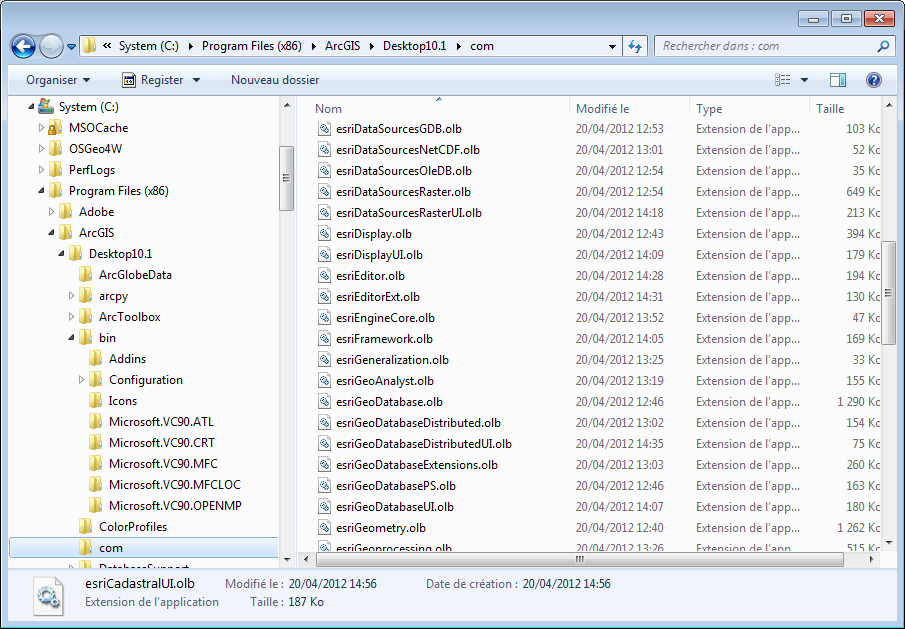
\includegraphics[width=0.70\textwidth]{img/cours/com_arcgis.png}
	\caption{Interfaces com installées avec ArcMap}
\end{figure}

Parmi ces bibliothèques, notons \textbf{esriSystem} qui est celle de plus bas niveau, \textbf{esriGeometry} qui permet de manipuler la géométrie des entités géographiques, \textbf{esriGeodatabase} pour accéder aux données stockées sous forme d'une géodatabase, \textbf{esriServer} qui permet de se connecter à un serveur ArcGIS for Server et d'exploiter les ressources qu'il diffuse, \textbf{Server} pour consommer des web services proposés par des serveurs ArcGIS, \textbf{esriCarto} pour la création et l'affichage de cartes, \textbf{esriNetworkAnalysis} pour la création d'une topologie arc-nœud et son exploitation, \textbf{esriAnimation} pour la création d'animations temporelles dans ArcMap, ArcScene et ArcGlobe, etc.

Le framework .Net utilise, contrairement à VBA par exemple, des bibliothèques compatibles (des \textit{assemblies}) qui font référence aux bibliothèques de l'API ArcObjects. Ce sont ces assemblies qu'il convient de référencer dans un projet .Net.


\subsection{Les SDKs Runtime}
\textbf{ArcGIS Runtime} est une nouvelle solution de développement apparue avec le version 10.1 d'ArcGIS. Il s'agit en fait d'un ensemble de 6 SDKs de bas niveau s'adressant chacun à des plateformes d'exécution spécifiques : Android, iOS, Windows Phone, Linux, OS X ou Windows.

\begin{figure}[H]
	\center 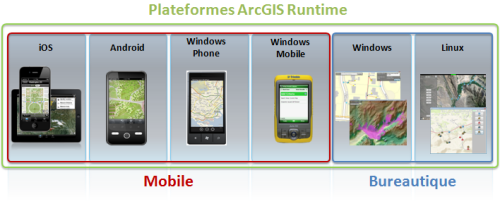
\includegraphics[width=0.6\textwidth]{img/cours/arcgis_runtime-1.png}
	\caption{Possibilités d'applications natives ArcGIS Runtime}
\end{figure}

Indépendant de tout objet COM, ces SDKs s'appuient sur un noyau commun : le \textbf{Runtime core} écrit en C++. Le noyau Runtime expose ses fonctionnalités à travers des services REST, sur le principe d'un ArcGIS for Server exposant ces services en REST. Cette architecture basée sur des services permet l'exécution asynchrone de plusieurs tâches simultanément. 

\begin{figure}[H]
	\center 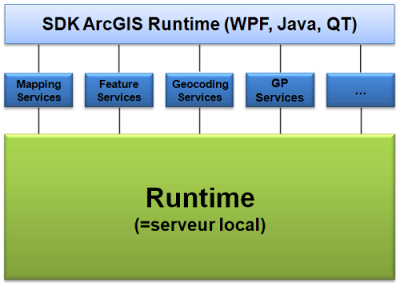
\includegraphics[width=0.6\textwidth]{img/cours/arcgis_runtime-2.png}
	\caption{Noyau ArcGIS Runtime}
\end{figure}

Les services REST Runtime sont consommés par des APIs Java, .Net ou C++ dont le fonctionnement est très proche de celui des APIs web d'ArcGIS, ce qui permettra au développeur de passer plus facilement d'un développement bureautique à un développement web. Les API Runtime sont également capable de communiquer directement avec des services ArcGIS Online ou ArcGIS for Server.

6 SDKs permettent enfin au développeur de manipuler les APIs Runtime :
\begin{itemize}
	\item ArcGIS Runtime SDK for Android
	\item ArcGIS Runtime SDK for iOS
	\item ArcGIS Runtime SDK for Java
	\item ArcGIS Runtime SDK for Mac OS X
	\item ArcGIS Runtime SDK for .Net
	\item ArcGIS Runtime SDK for .Qt
\end{itemize}

Les SDKs ArcGIS Runtime permettent de développer des applications natives ou des extensions sur des applications existantes. Ils permettent de créer des processus de géotraitement ainsi que de manipuler de nouveaux types de données non accessible en standard dans ArcGIS.

En terme de fonctionnalités, ArcGIS Runtime propose des capacités en cartographie, utilisation couplée de données locales et web, analyse, collecte de données, géocodage,  etc. Il permet de travailler en mode connecté et déconnecté.


\subsection{L'API Python}
Les développements python répondent à deux besoins : d'une part celui d'automatiser les processus de traitements de l'information géographique, d'autre part celui d'écrire des traitements personnalisés. Il s'agit de développement de moins bas niveau qu'avec les ArcObjects ou ArcGIS Runtime. Le développeur peut recourir à un environnement Python indépendant ou bien intégré à ArcGIS.

Ils permettent de produire des scripts de géotraitement qui peuvent être intégrés sous forme d'outils dans l'interface d'ArcGIS bureautique, ou encore être publiés sous forme de services par ArcGIS for Server.

L'API Python est apparue avec la version 9 d'ArcGIS et était complétée dès le départ d'un environnement de développement et d'exécution intégré à ArcMap. Le périmètre fonctionnel de ce SDK a été jusqu'à la version 10 celui de l'environnement de géotraitements. Depuis la version 10, le périmètre a été étendu : il est maintenant possible de manipuler les documents, leurs couches d'objets (géographiques ou graphiques) ainsi que leur représentation ce qui, combiné aux capacités classiques de géotraitements permet de concevoir des processus automatiques de création et de mise à jour de carte. 

Le SDK Python est parfaitement intégré aux autres outils de géotraitements : la fenêtre de commandes Python permet d'exécuter chacun d'entre eux. C'est plus qu'une ligne de commande puisqu'il est possible de coder des blocs d'instructions. Un modèle conçu avec ModelBuilder est par ailleurs exportable sous forme d'un script Python. Il est également possible de développer ex nihilo un nouvel outil pour ArcToolBox puis de l'ajouter en tant que script. Enfin les compléments python permettent un déploiement aisée et mieux intégré à l'interface d'ArcGIS. Ce dernier mode de diffusion nécessite l'utilisation d'un assistant\footnote{https://www.arcgis.com/home/item.html?id=5f3aefe77f6b4f61ad3e4c62f30bff3b}.

\begin{figure}[H]
	\center 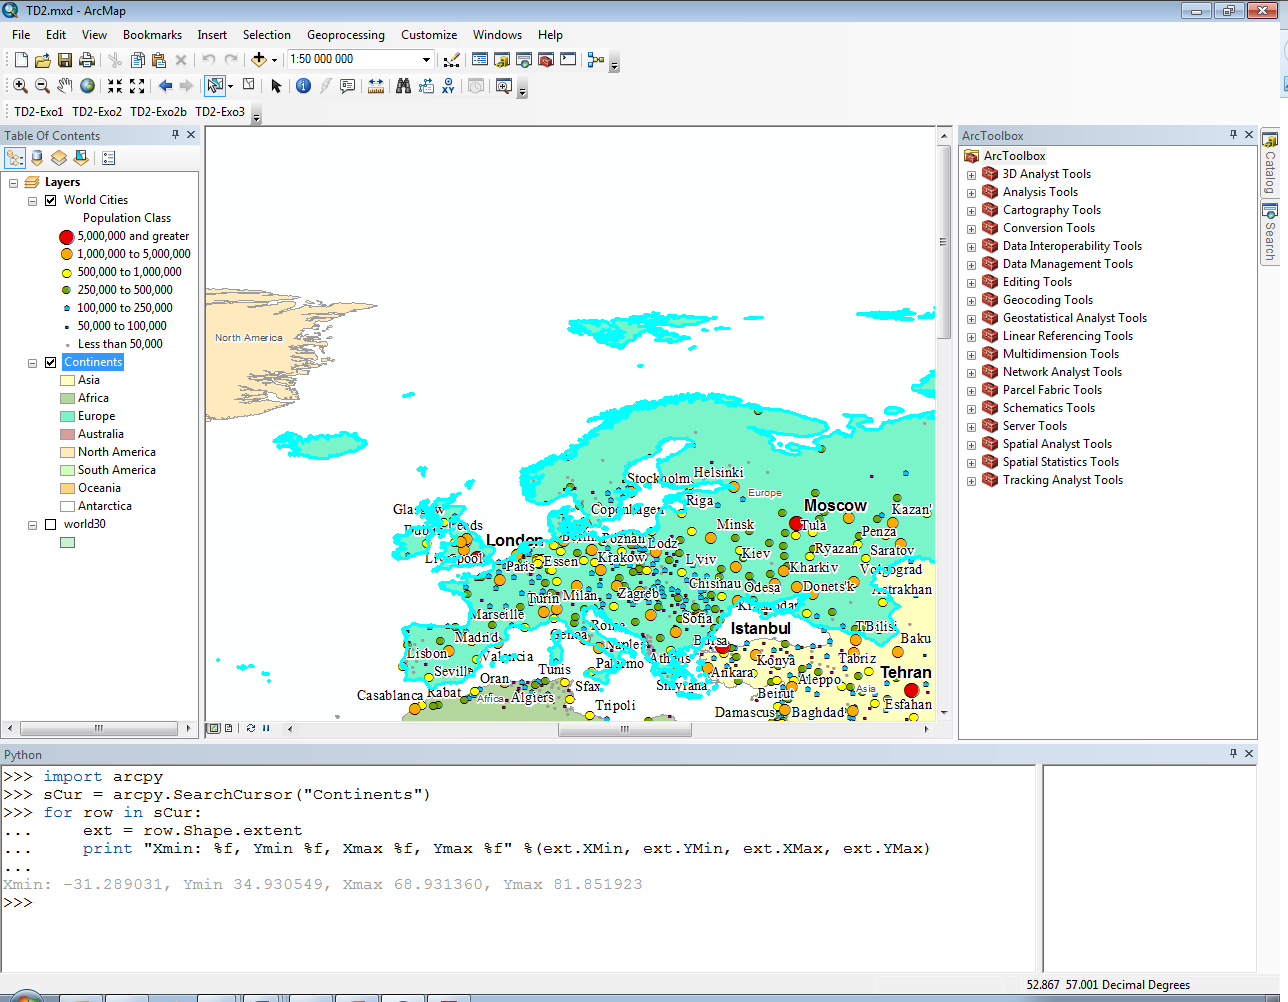
\includegraphics[width=0.6\textwidth]{img/cours/console_python.png}
	\caption{Console Python d'ArcMap}
\end{figure}

L'API Python repose sur un site-package nommé \textbf{ArcPy}, qui est en fait une version étendue du module arcgisscripting utilisé en version 9. Pour être tout à fait exact, ArcPy intègre arcgisscripting mais propose en plus un accès à des classes d'objets, à une bibliothèque de fonctions, ainsi qu'à des modules SIG spécifiques (arcpy.mapping, arcpy.sa spatial analyst, arcpy.ga géostatistical analyst).

Cette API présente un potentiel intéressant dans la mesure où elle peut être utilisée conjointement avec d'autres API Python (NumPy par exemple).


\subsection{Les développements web}
La tendance est aujourd'hui au développement web rapide à base d'APIs simplifiées et de templates d'application. Les solutions Esri n'échappent pas à la règle et permettent de déployer des applications web sans avoir à écrire une seule ligne de code. 

Derrière ces solutions faciles à mettre en oeuvre, des APIs plus fondamentales permettent de consommer les services web exposées en REST par le serveur ArcGIS. Esri a fournit 3 APIs pour développer des clients riches : l'API Javascript for ArcGIS, l'API Flex for ArcGIS et l'API Silverlight for ArcGIS. Mais aujourd'hui, seule l'API Javascript est encore maintenue par la firme américaine, les technologies Flex et Silverlight n'étant plus trop d'actualité dans le monde du web.

Le développeur peut toujours reprendre la main sur ces APIs, pour améliorer le code ou développer ses propres solutions.


\subsubsection{Utilisation d'un générateur d'applications web}
Sur le même principe que l'AppStudio for ArcGIS, un générateur d'application en ligne permet de créer des applications web sans écrire une seule ligne de code : \textbf{Web Appuilder for ArcGIS}. Cette solution est bien entendu limitée en terme de personnalisation.

Ce composant se base sur l'utilisation de modèles et widgets, ainsi que sur la personnalisation des styles et thèmes pour réaliser des applications web fonctionnelles et attrayantes. En arrière plan, du code HTML5/Javascript, en utilisant l'API ArcGIS est généré. Le développeur peut bien entendu toujours reprendre la main sur ce code pour étendre les fonctionnalités proposées en standard par Esri.

\begin{figure}[H]
	\center 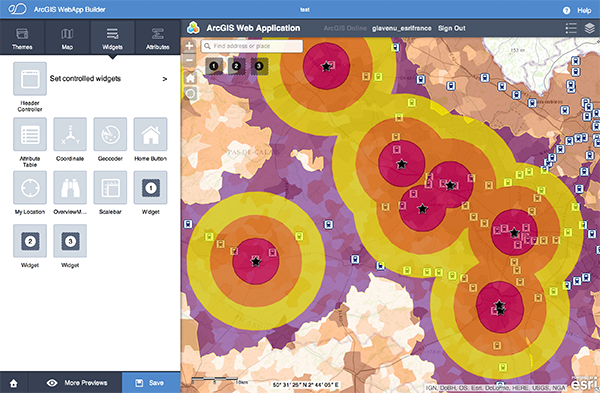
\includegraphics[width=0.70\textwidth]{img/cours/web_appbuilder.png}
	\caption{Choix des widgets dans Web AppBuilder for ArcGIS}
\end{figure}


\subsubsection{Configuration de modèles d'applications}
Pour simplifier le développement d'applications sur des clients riches courants, Esri fournit toujours des modèles d'applications configurables pour Flex et Silverlight, même si les API derrière ces technologies n'évoluent plus. 

\textbf{ArcGIS Viewer for Silverlight} permet de parcourir des assistants qui vous aident à ajouter de manière interractive les composants de votre choix dans votre application (carte créée sur ArcGIS Online, services cartographiques). Il est possible d'obtenir une application cartographique Silverlight prête à être déployée en quelques minutes sans écrire beaucoup de code.

De manière semblable, \textbf{ArcGIS Viewer for Flex} est un générateur pour créer des applications avec Adobe Flex. Cette visionneuse offre une multitude de widgets et vous permet de consommer des services ArcGIS Online et/ou ArcGIS for Server.


\subsubsection{Utilisation d'une API web}
Pour aller plus loin en terme de personnalisation, le développeur va utiliser l'une des APIs web d'Esri : 
\begin{itemize}
	\item \textbf{les API Flex ou Silverlight} qui permettent de travailler à partir de modèles et fournissent des solutions évoluées mais nécessite qu'un plugin soit installé sur le navigateur du client;
	\item l'\textbf{API JavaScript} éxécuté côté client sans plugin;
	\item ou encore l'\textbf{API Esri Leaflet} qui est un dérivé de la bibliothèque libre Javascript Leaflet pour en faciliter l'utilisation
\end{itemize}

Toutes ces APIs exploitent l'API REST d'ArcGIS for Server. L'API Javascript est assurément la plus utilisée et la seule garantie d'être maintenue sur le long terme. Depuis la version 4.0, la 3D est complètement intégrée à l'API et sa gestion est identique à celle de la 2D.

\begin{figure}[H]
	\center 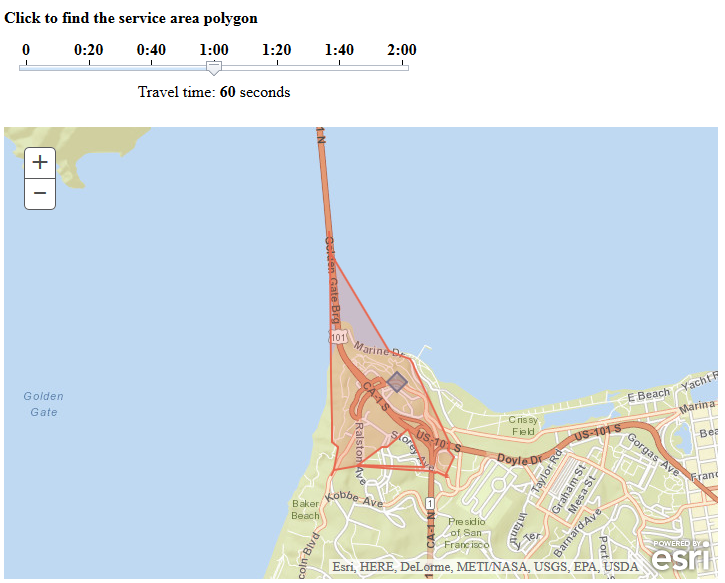
\includegraphics[width=0.32\textwidth]{img/cours/api_javascript.png}
	\caption{Exemple d'application web SIG basée sur l'API Javascript}
\end{figure}

Pour aller au-delà des capacités de ces APIs ou exposer une logique métier personnalisée, le développeur a encore la possibilité d'utiliser des \textbf{extensions d'objet serveur (SOE)} ou des \textbf{intercepteurs d'objet serveur (SOI)}. Ces extensions côté serveur se basent sur les ArcObjects et permettent au développeur expérimenté de profiter de toutes les fonctionnalités d'un serveur ArcGIS dans une application web.


\subsection{Les API mobiles}
C'est assurément un secteur d'activités en pleine croissance. Esri propose depuis plusieurs années l'application ArcPad destinée aux collecteurs de données géographiques sur le terrain. Celle-ci tend aujourd'hui à être supplantée par d'autres types d'applications conçues naturellement pour interagir avec des serveurs : il s'agit du produit ArcGIS Mobile. Ces applications s'exécutent en environnement Windows, Windows mobile, Windows Phone, Androïd ou encore iOS. Chacune de ces applications est personnalisable à l'aide d'un SDK dédié.

Le SDK d'ArcGIS Mobile est un SDK .Net composé d'un certain nombre d'assemblies (dll). Le SDK comprend deux parties : le noyau (Core SDK) et l'application (Application SDK), la partie application étant cliente de la partie noyau. Le core SDK est fourni par l'assembly ESRI.ArcGIS.Mobile.dll, l'application SDK par l'assembly ESRI.ArcGIS.Mobile.Client.dll.

Notons enfin que les SDKs Runtime permettent aujourd'hui de développer des applications pour mobile (ArcGIS Runtime SDK for Android, ArcGIS Runtime SDK for iOS). Les techniques et technologies mises en oeuvre pour développer des applications bureautiques et mobiles sont ainsi les mêmes et parler de développements pour mobiles comme un type de développement particulier a de moins en moins de sens lorsque l'on utilise des outils Esri.

 
\subsection{Le générateurs d'applications}
Afin de faciliter le travail de création d'application, Esri travaille sur des outils de génération d'applications à partir de modèles, ne nécessitant l'écriture d'aucune ligne de code. Cette solution, \textbf{AppStudio for ArcGIS} permet de créer des applications multi-plateforme (Android, iOS, Linux, Mac ou Windows).

Ce générateur permet aux non-développeurs de concevoir des applications à partir de modèles et de widgets standard, ainsi que de services ArcGIS Online ou ArcGIS for Server. Une fois l'application configurée, AppStudio for ArcGIS prend en charge sa compilation sur les différentes plateformes cibles. 

Cet outil intéresse néanmoins les développeurs puisqu'ils pourront étendre un modèle existant ou construire leur propre modèle à l'aide de la programmation. AppStudio for ArcGIS est basé sur l'API QML du SDK ArcGIS Runtime for Qt.

\begin{figure}[H]
	\center 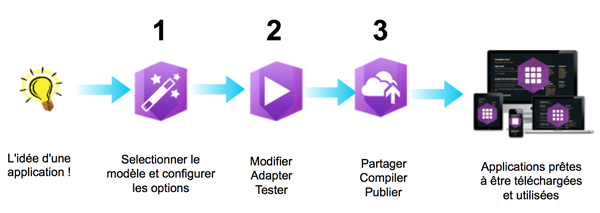
\includegraphics[width=0.70\textwidth]{img/cours/AppStudio_for_ArcGIS-2.png}
	\caption{Processus de création d'application avec AppStudio for ArcGIS}
\end{figure}


\subsection{Arcade}
Arcade est un langage développé par Esri fin 2016 pour gérer la symbologie dans les applications de sa plateforme. Il permet d'exécuter des expressions évoluées (opérations mathématiques, conditions, boucles...) pour contrôler le rendu d'entités ou le texte d'étiquettes. Si la modification de la symbologie est quelque chose que toutes les applications ou développements permettent déjà de faire, la grande force d'Arcade réside dans sa portabilité : le même script Arcade pourra être lu dans ArcGIS Pro, dans ArcGIS Online, dans une application web développée avec l'API Javascript ou encore dans un outil basé sur les SDKs Runtime.



\end{document}

